\documentclass[../main.tex]{subfiles}
\graphicspath{{\subfix{../assets/}}}

\begin{document}
\subsection{Mediu de dezvoltare și generalități}
Procesorul împreună cu celelalte circuite au fost proiectate în \acrshort{vhdl} în mediul de dezvoltare
\emph{Active-HDL Student Edition}. \emph{Active-HDL} pune la dispoziție instrumente pentru compilarea și
simularea codului \acrshort{vhdl} și Verilog. \acrshort{vhdl} este un limbaj de programare hardware. Înseamnă
că un program \acrshort{vhdl} nu poate fi rulat pe un calculator, trebuie încărcat pe o placă \acrshort{fpga},
care pe baza codului va genera circuitele și conexiunile dintre ele. E o metodă rapidă de prototipare și testare
pentru noi dispozitive hardware dar în același timp versiuni ieftine de plăci pot fi folosite în loc de
proiectarea circuitelor electronice dedicate în anumite produse.

Proiectul coține următoarele circuite ce vor fi explicate în detaliu și care pot fi observate în figura 
\ref{fig:main_block_diagram}:
\begin{itemize}
    \item Procesor cu arhitectură \acrshort{subleq}
    \item Memorie cache cu mapare directă, \emph{write-back} cu \emph{write-allocate}
    \item Memorie RAM \emph{single port}, citire asincronă și scriere sincronă
    \item Circuit de arbitrare cu prioritate
    \item Circuit de sincronizare print \emph{handshaking}
    \item Bistabil de tip D folosit în implementarea circuitului de sincronizare (nu apare în figura \ref{fig:main_block_diagram})
\end{itemize}

\begin{figure}[h]
    \centering
    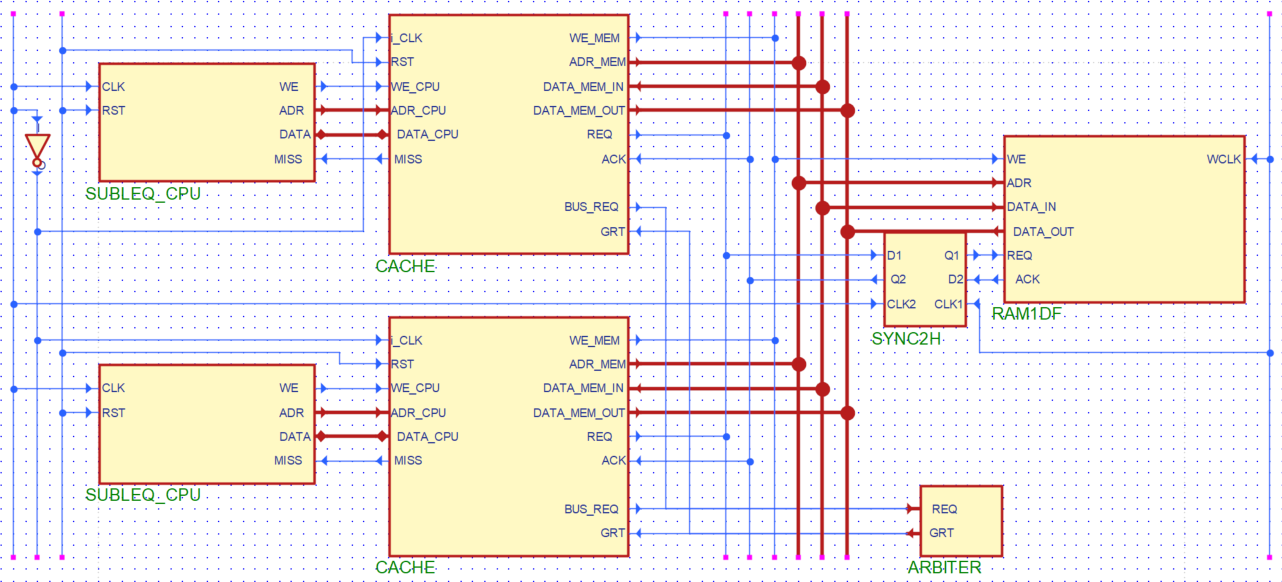
\includegraphics[width=0.9\textwidth]{main_block_diagram.png}
    \caption{Schema bloc generală}
    \label{fig:main_block_diagram}
\end{figure}

Codul \acrshort{vhdl} cu entitățile circuitelor se află la anexa \ref{appendix:entities}. O entitate e un noțiune \acrshort{vhdl}
care descrie porturile și pinii unui circuit. Asemenea unei interfețe care poate avea mai multe implementări, o entitate poate
avea mai multe arhitecturi. Aproape toate entitățile au și parametrii generici pentru a controla ușor numărul liniilor de date,
numărul liniilor de adresă și dimensiunea memoriilor. Fiecare port sau pin are un prefix în nume pentru a specifica dacă este
de intrare, de ieșire sau de intrare-ieșire.

\subsection{Implementarea procesorului SUBLEQ}
Arhitectura \acrshort{subleq} a fost aleasă din cauza popularității ei în mediul online și din cauza simplității.
Procesorul e implementat ca un automat cu stări finite care păstrează o stare internă cu informațiile necesare
pentru a putea funcționa. În figura \ref{fig:cpu_state} se pot observa stările și tranzițiile dintre acestea.
Majoritatea stărilor și desigur, majoritatea instrucțiunilor din \emph{pipeline} sunt cele de tip \emph{fetch}.
Executarea unei singure instrucțiuni \acrshort{subleq} presupune 5 operații \emph{fetch}, o operație \acrshort{alu},
o operație de scriere și încă una de decizie. Ca optimizare se verifică dacă noua valoare ce urmează să fie scrisă
este diferită de cea care există deja la acea adresă, caz în care se sare peste operația de scriere, fiind
redundantă.

\begin{figure}[h]
    \centering
    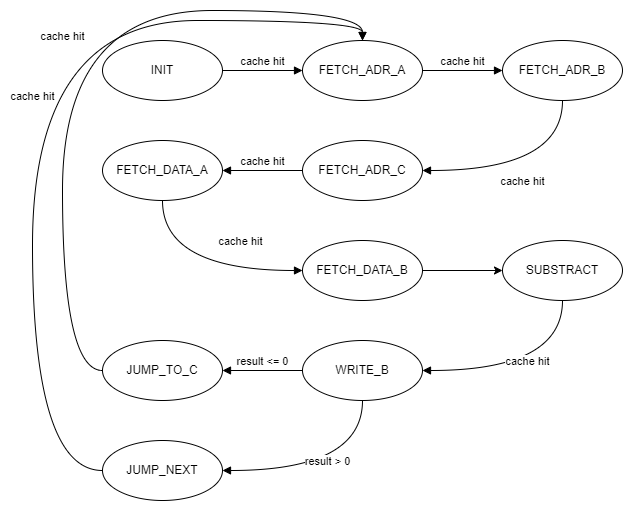
\includegraphics[width=0.9\textwidth]{cpu_state.png}
    \caption{Diagrama de stare a procesorului}
    \label{fig:cpu_state}
\end{figure}

Semnalele procesorului sunt, după cum se văd în figura \ref{fig:main_block_diagram} și la anexa \ref{appendix:entities}:
\begin{itemize}
    \item i\_CLK -- semnal de intrare -- semnalul de \emph{clock}
    \item i\_RST -- semnal de intrare -- semnal de reset, are același efect cu stare INIT din figura \ref{fig:cpu_state}
    \item i\_MISS -- semnal de intrare -- `1' în cazul unui \emph{cache miss} și `0' pentru un \emph{cache hit}
    \item o\_WE -- semnal de ieșire -- `1' pentru operația de scriere, `0' pentru citire
    \item o\_ADR -- semnal de ieșire -- adresa de la care se citește sau în care se scrie
    \item io\_DATA -- semnal de intrare ieșire -- contine datele ce vor fi scrise sau citite de la adresa specificată
\end{itemize}

\end{document}